\setkeys{Gin}{width=0.9\textwidth}
\section{Results}\label{sec:results}
Four circuits were assembled and analyzed using a function generator to apply a stimulus, and an oscilloscope to measure the output of the system over the input. A detailed diagram of the circuits which produced these outputs can be referenced in the lab manual \cite{lab-manual}.
\begin{figure}[htbp]
	\centering
	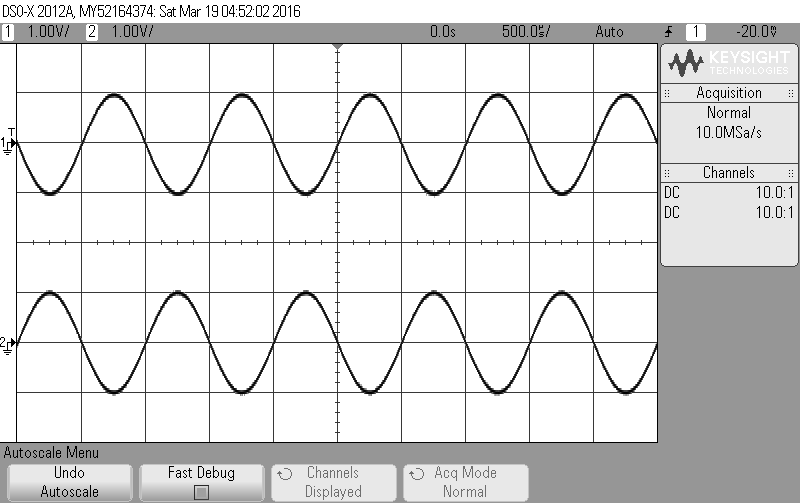
\includegraphics{response-inverter}
	\label{fig:inverter}
	\caption{Input versus output of inverter circuit}
\end{figure}

\begin{figure}[htbp]
	\centering
	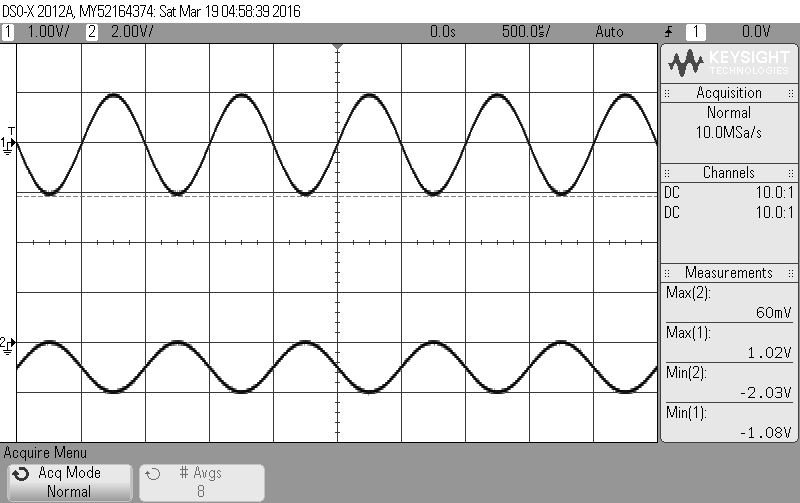
\includegraphics{response-adder}
	\label{fig:adder}
	\caption{Input versus output of adder circuit}
\end{figure}

\begin{figure}[htbp]
	\centering
	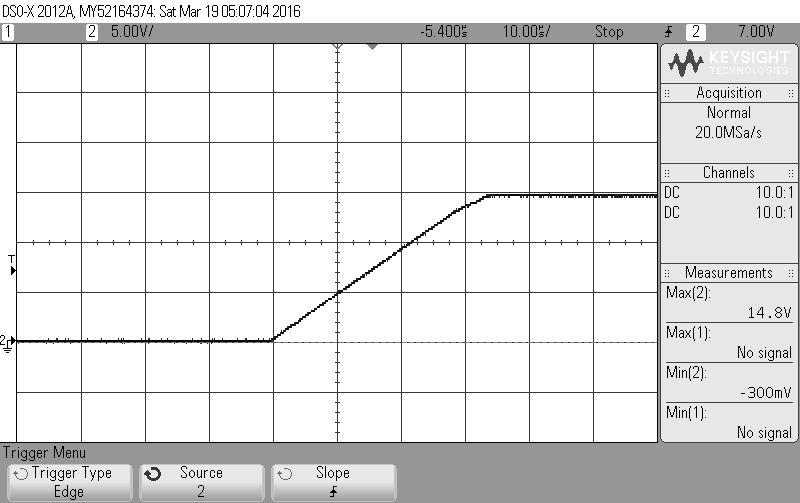
\includegraphics{response-integrator}
	\label{fig:integrator}
	\caption{Input versus output of integrator circuit}
\end{figure}

\begin{figure}
	\centering
	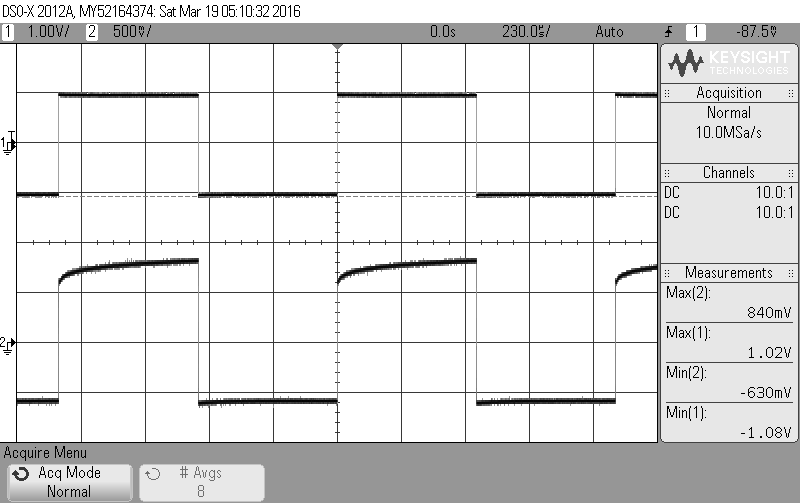
\includegraphics{response-first-order}
	\label{fig:first-order}
	\caption{Input versus output of first order system with an integrator}
\end{figure}

\clearpage
